\subsection{Mutual information as similarity for hierarchical clustering}
\label{subsec:analysis-clustering-mi}

\parencite{granadosDistributedDynamicIntracellular2018} describe a mutual information algorithm.

(Copy some of the maths here, explain it a bit)

% TODO: Re-do with better data, better code, etc.
% Or just give up with it because I've shown that mutual information doesn't work so well?
We can see mutual information as a measure for a classification model -- in the same vein as precision, recall, etc.  This is because mutual information produces a value that (indirectly) represents the similarity between two sets of time series data, based on computing confusion matrices via bootstrapping.  To be accurate, mutual information asks the question of to what extent it is possible to distinguish two typical time series sampled from each of two sets of time series.

I can then compute the mutual information between pairs of strains in a dataset, then use the mutual information as a distance measure to produce hierarchical clustering between the strains.

I divide this into three cases:
\begin{enumerate}
\item Include oscillatory time series only.
\item Include non-oscillatory time series only.
\item Include all time series.
\end{enumerate}

Unless otherwise noted, I restrict the range (time points 25 - 168), detrend using a sliding window of 45 time points, and featurise using catch22.  Scaling the features is already included in the mutual information code, and thus not repeated before.  With the mutual information code, I use 1000 bootstraps.

\subsubsection{Causton strains (19979)}
\label{sec:org14969a0}

This is the older experiment with the defective CEN.PK strain but with more cells in total.

Oscillatory only
\label{sec:org468bf6f}

Distance matrix

\begin{center}
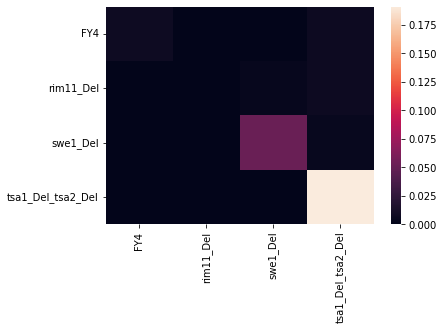
\includegraphics[width=.9\linewidth]{MIHierClust_19979_osc_distmatrix.png}
\end{center}

Dendrogram (UPGMA)

\begin{center}
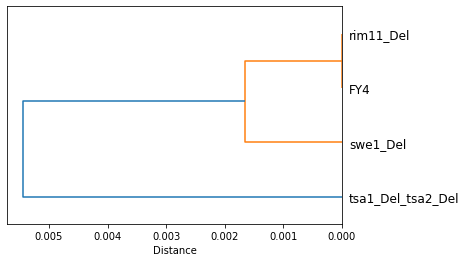
\includegraphics[width=.9\linewidth]{MIHierClust_19979_osc_dendrogram.png}
\end{center}

This suggests that the Causton strains' time traces are very similar to each other.

Switching to using time series as features did not change the values by much -- they were still zero or near-zero.

Non-oscillatory only
\label{sec:org0984c97}

Distance matrix

\begin{center}
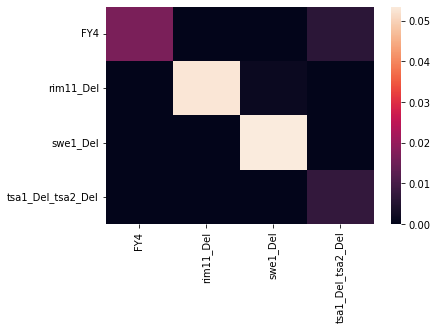
\includegraphics[width=.9\linewidth]{MIHierClust_19979_nosc_distmatrix.png}
\end{center}

Dendrogram (UPGMA)

\begin{center}
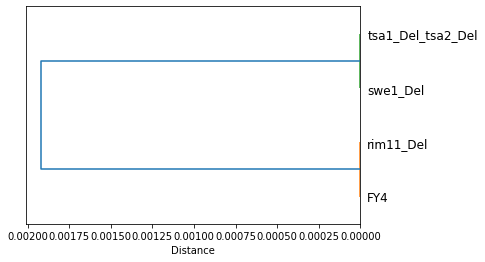
\includegraphics[width=.9\linewidth]{MIHierClust_19979_nosc_dendrogram.png}
\end{center}

This suggests that non-oscillatory time series are similar between strains, which justifies removing them from the feature matrix when performing UMAP in (Identifying the most important catch22 features for classification).  Additionally, removing non-oscillatory time series make biological sense -- we want to see whether single-cell flavin oscillations differ between the strains, and it doesn't make sense to have non-oscillatory time series from potentially dead cells, technical issues, or noise in the data.

All cells
\label{sec:org0854ace}

Distance matrix

\begin{center}
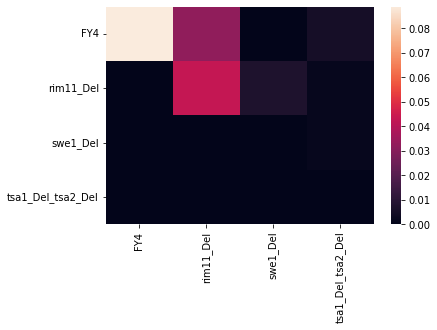
\includegraphics[width=.9\linewidth]{MIHierClust_19979_all_distmatrix.png}
\end{center}

Dendrogram (UPGMA)

\begin{center}
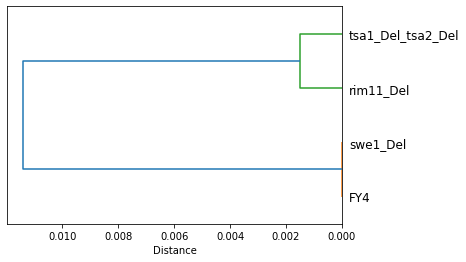
\includegraphics[width=.9\linewidth]{MIHierClust_19979_all_dendrogram.png}
\end{center}

The small distances when all cells are included further justifies the removal of non-oscillatory time series.

\subsubsection{Causton strains (20212)}
\label{sec:orgcc0d5be}

This is the newer experiment with the correct CEN.PK strain from Peter Kötter, but fewer cells in total.

Oscillatory only
\label{sec:org803a4be}

Distance matrix

\begin{center}
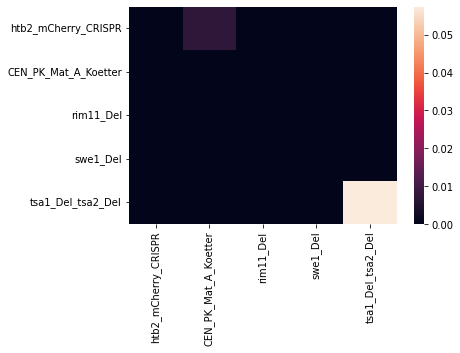
\includegraphics[width=.9\linewidth]{MIHierClust_20212_osc_distmatrix.png}
\end{center}

Dendrogram (UPGMA)

\begin{center}
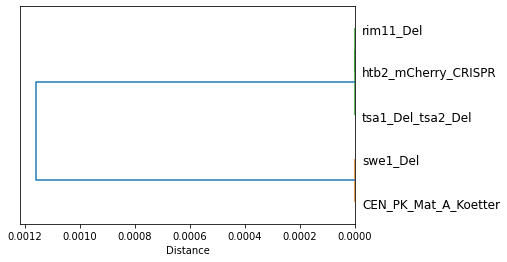
\includegraphics[width=.9\linewidth]{MIHierClust_20212_osc_dendrogram.png}
\end{center}

Same story, we can't tell the strains apart.

\subsubsection{BY4741 vs zwf1$\Delta$}
\label{sec:org7a4d63f}

Oscillatory only
\label{sec:org3fdb03d}

Distance matrix

\begin{center}
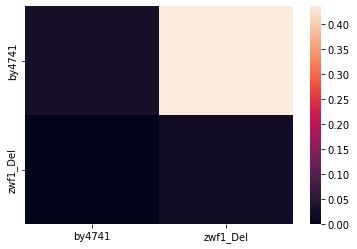
\includegraphics[width=.9\linewidth]{MIHierClust_20016_osc_distmatrix.png}
\end{center}

This suggests that there is a considerable difference between these two strains.  Given how classifiers tend to be able to tell apart these strains very well, it is not surprising.

Switching to using time series as features gives a median MI of 0.46 (median 0.46368494, IQR 0.40093307 -- 0.51805235), which isn't a big change from before.

\subsubsection{Remarks}
\label{sec:orga7cc61d}

\begin{itemize}
\item MI with itself: some cases are non-zero (or, not close to zero).  Does this mean that there is enough variety within the dataset concerned that there is a risk of overfitting?
\item This is probably an additional line of evidence to confirm that there is no real difference between Causton strains in terms of their single-cell flavin oscillations.
\item Potential extension: to wild-type/prototrophic strains in different glucose concentrations.
\end{itemize}
